\documentclass{article}\usepackage[]{graphicx}\usepackage[]{color}
%% maxwidth is the original width if it is less than linewidth
%% otherwise use linewidth (to make sure the graphics do not exceed the margin)
\makeatletter
\def\maxwidth{ %
  \ifdim\Gin@nat@width>\linewidth
    \linewidth
  \else
    \Gin@nat@width
  \fi
}
\makeatother

\definecolor{fgcolor}{rgb}{0.345, 0.345, 0.345}
\newcommand{\hlnum}[1]{\textcolor[rgb]{0.686,0.059,0.569}{#1}}%
\newcommand{\hlstr}[1]{\textcolor[rgb]{0.192,0.494,0.8}{#1}}%
\newcommand{\hlcom}[1]{\textcolor[rgb]{0.678,0.584,0.686}{\textit{#1}}}%
\newcommand{\hlopt}[1]{\textcolor[rgb]{0,0,0}{#1}}%
\newcommand{\hlstd}[1]{\textcolor[rgb]{0.345,0.345,0.345}{#1}}%
\newcommand{\hlkwa}[1]{\textcolor[rgb]{0.161,0.373,0.58}{\textbf{#1}}}%
\newcommand{\hlkwb}[1]{\textcolor[rgb]{0.69,0.353,0.396}{#1}}%
\newcommand{\hlkwc}[1]{\textcolor[rgb]{0.333,0.667,0.333}{#1}}%
\newcommand{\hlkwd}[1]{\textcolor[rgb]{0.737,0.353,0.396}{\textbf{#1}}}%
\let\hlipl\hlkwb

\usepackage{framed}
\makeatletter
\newenvironment{kframe}{%
 \def\at@end@of@kframe{}%
 \ifinner\ifhmode%
  \def\at@end@of@kframe{\end{minipage}}%
  \begin{minipage}{\columnwidth}%
 \fi\fi%
 \def\FrameCommand##1{\hskip\@totalleftmargin \hskip-\fboxsep
 \colorbox{shadecolor}{##1}\hskip-\fboxsep
     % There is no \\@totalrightmargin, so:
     \hskip-\linewidth \hskip-\@totalleftmargin \hskip\columnwidth}%
 \MakeFramed {\advance\hsize-\width
   \@totalleftmargin\z@ \linewidth\hsize
   \@setminipage}}%
 {\par\unskip\endMakeFramed%
 \at@end@of@kframe}
\makeatother

\definecolor{shadecolor}{rgb}{.97, .97, .97}
\definecolor{messagecolor}{rgb}{0, 0, 0}
\definecolor{warningcolor}{rgb}{1, 0, 1}
\definecolor{errorcolor}{rgb}{1, 0, 0}
\newenvironment{knitrout}{}{} % an empty environment to be redefined in TeX

\usepackage{alltt}
\usepackage{amsmath}
\usepackage{makecell}
\setcellgapes{5pt}
\usepackage{graphics}
\usepackage{multirow}
\usepackage{multicol}
\usepackage[cm]{fullpage}
\graphicspath{ {./images/} }
\usepackage{titling}
\usepackage[table]{xcolor}
\usepackage[mathscr]{euscript}
\usepackage{mathrsfs}
\usepackage{ulem, cancel}
\usepackage{boldline}

\title{COSC 6323 - Statistical Methods in Research\\Project Phase - 3\\}

\author{%
    Members: Team-8 \\\\
    1. Farah Naz Chowdhury,    \texttt{ID:1798957}, \texttt{fchowdhury4@uh.edu}      \vspace{2pt} \\
    2. Md Rafiqul Islam Rabin, \texttt{ID:1797648}, \texttt{mrabin@central.uh.edu}   \vspace{2pt} \\
    3. S M Salah Uddin Kadir , \texttt{ID:1800503}, \texttt{ssalahuddinkadir@uh.edu} \vspace{2pt} \\
}

\date{May 02, 2019.}
\IfFileExists{upquote.sty}{\usepackage{upquote}}{}
\begin{document}

\maketitle
\par{\textbf{Contributions}: We sit together to discuss the requirement and task distribution. We divided task equally among us and agreed to support each other. The contribution status - Data Analysis (All Faculty - Rabin, XD only - Prity, Matched XD - Salah Uddin), Model (TableS4 - Rabin, TableS5 - Prity, TableS6 - Salah Uddin), Fig5 (5A+5B - Salah Uddin, 5C+5D - Rabin), and Report (Rabin, Prity, Salah Uddin). We always shared our progress/problem with each other and helped during implementation. We distributively contributed to our created git repository for the project. As we all completed our tasks and actively involved with each other all the times, we equally contributed to the project.}

%Fig. 5
\newpage
\section*{\underline{Fig. 5:}}
\begin{center}
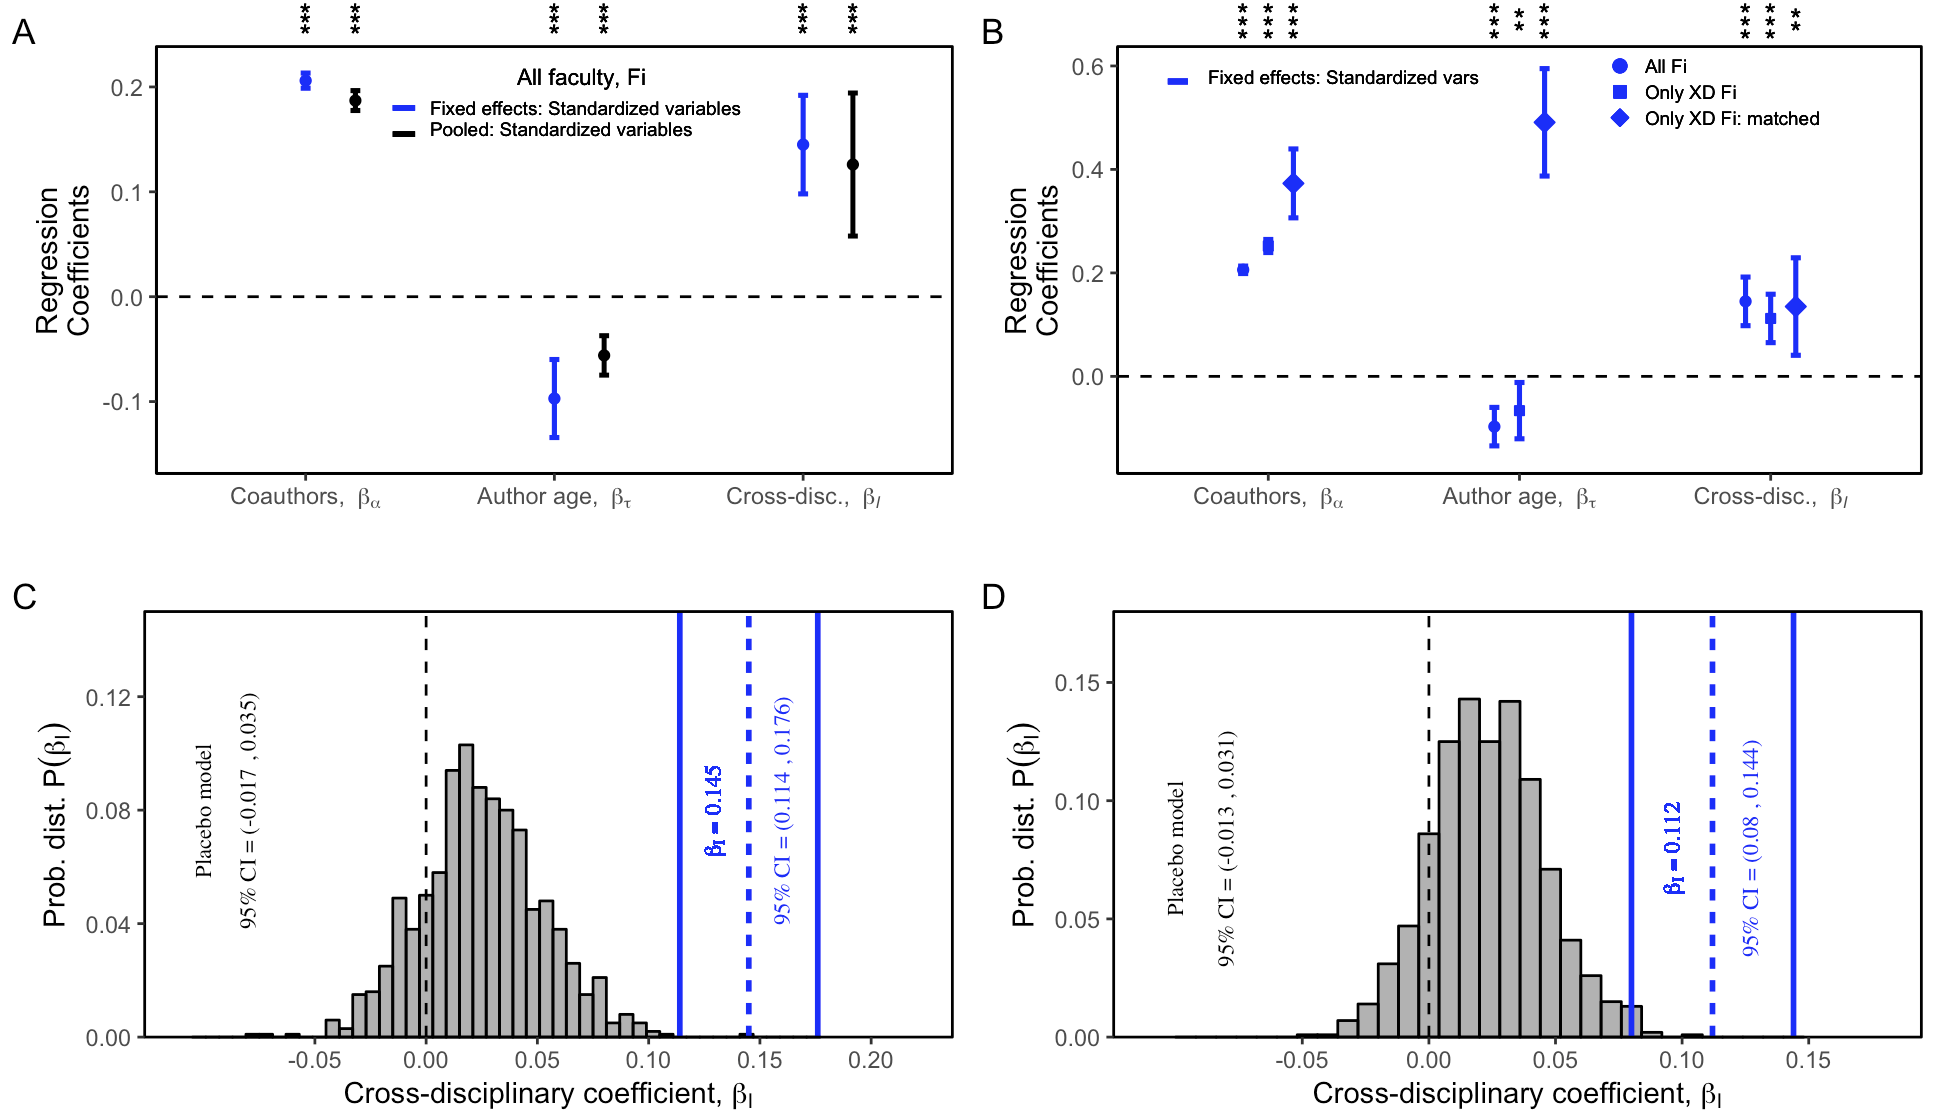
\includegraphics[scale=0.5]{Fig5.png}
%\newline
\par{\textbf{Fig. 5. Career panel regression model.}}
\end{center}
\subsection*{\underline{Description of figure content:}}
\par{
($\textbf{5A, 5B}$) Co-authors (${{\beta}_a}$), Author age (${{\beta}_{\tau}}$), and Cross-disciplinary indicator of publication(${\beta}_I$) are three principal explanatory variables included in the fixed effect $\mathcal{F}$ career model. Regression coefficients are given in y-axis and explanatory variables are given in x-axis. Parameter estimates are given in TableS4, TableS5 and TableS6. Fig 5A shows the model estimates for those three explanatory variables and represents the relationship between explanatory variables and citation impact. The green color indicates fixed standardized effect and black color is pooled standardized effect. Fig 5B shows the fixed effect model estimates for (i) all faculty, (ii) only cross-disciplinary faculty, and (iii) cross-disciplinary matched pair faculty. The circle shape for all faculty, square shape for xd only faculty and diamond shape for matched xd faculty. ($\textbf{5C, 5D}$) The placebo randomization has been taken place to explore the spurious correlations. To check the robustness of panel regression model, in this regards, we shuffled the ${I}^{XD}_{i,p}$ value across the data set without replacement. For random 1000 faculty, we ran placebo randomization and repeat this 1000 times and calculate the value of ${\beta}_I$. The solid blue line in left side indicates the ${\beta}_I$ value of third column of TableS4 and dashed blue line indicates the 95\% confidence interval (CI). The x-axis shows the ${\beta}_I$ value and y-axis shows the probability distribution in specified binwidth, calculated by count divided by total observation. Fig 5C shows the distribution of the placebo estimates $P({\beta}_I)$ for all faculty $\mathcal{F}_i$, on the other hand, Fig 5D shows the distribution of the placebo estimates $P({\beta}_I)$ for cross-disciplinary faculty $\mathcal{F}_{XD}$. The levels of statistical significance ($p-value$) are as follows: **$\textit{p}$ $\leq$ 0.01, ***$\textit{p}$ $\leq$ 0.001.
}
\subsection*{\underline{Observations, conclusions, and hypotheses:}}
\begin{description}
  \item[$\bullet$] Fig 5A. The relationship between career model explanatory variables and citation impact are shown in this figure: (i) There is a positive relationship between cross-disciplinary and citation impact that means the average cross-disciplinary publication is more highly cited than the average disciplinary publication. (ii) We also observe a positive relationship between team size and citation impact that means the increase of citation is associated with the increase of team size. (iii) But we observe a negative relationship between career age and citation impact that means the citation decrease with each career year. Additionaly, the estimates with xd only faculty and matched xd faculty are also consistent which indicates the sign of robustness.
  \item[$\bullet$] Fig 5B. The parameter estimates are consistent for co-authors and cross-disciplinary indicator, both positive with (i) all faculty, (ii) xd faculty, and (iii) matched xd faculty. On the other hand, the parameter estimates are not consistent for author age, as it is negative with (i) all faculty and (ii) xd faculty, but positive with (iii) matched xd faculty. This inconsistency of author age is because of the bias introducing by matched data of faculty's longitudinal profile.
  \item[$\bullet$] Fig 5C. The distribution of the placebo estimates $P({\beta}_I)$ is for all faculty $\mathcal{F}_i$. The paper claimed 0\% placebo estimates were larger than original estimates, but unfortunately we observed that around 10\% placebo estimates cross the original estimates. We believe this is for the random selection and we plot the distribution with filtering those overlap.
  \item[$\bullet$] Fig 5D. The distribution of the placebo estimates $P({\beta}_I)$ is for cross-disciplinary faculty $\mathcal{F}_{XD}$. The paper also claimed 0\% placebo estimates were larger than original estimates, but unfortunately we again observed that around 5\% placebo estimates cross the original estimates. We similarly believe this is for the random selection and we plot the distribution with filtering those overlap, as well.
\end{description}

%Table S4
\newpage
\section*{\underline{Table S4:}}
\begin{table}[h!]
  \begin{center}
  \resizebox{\columnwidth}{!}{%
  \begin{tabular}{l l l l l l }
  
    \hline
    \hline
    
  {} & \textbf{No Fixed Effects} & \textbf{No Fixed Effects} & \textbf{Fixed Effects} & \textbf{Fixed Effects}   \\
  {} &                           & \textbf{[Standardized]}   &                        & \textbf{[Standardized]}   \\
    
    \hline
    
    \textbf {Publication characteristics}\\
    
    \rowcolor{gray!33}
     {\#} of co-authors, $\beta_{\alpha}$ 
    & 0.284*** & 0.187***  & 0.312*** & 0.206***         \\
    {} 
    & (0.00718)   & (0.00474)    & (0.00547)   & (0.00361)           \\
    
    \rowcolor{gray!33}
    Career age, $\beta_{\tau}$ 
    & -0.00547***  & -0.0560***   & -0.00949***  & -0.0971***   \\
    {} 
    & (0.000919)   & (0.00940)    & (0.00182)   & (0.0186)     \\
    
    \rowcolor{gray!33}
    Cross-disciplinary indicator, $\beta_{I}$ 
    & 0.126***   & 0.126***     & 0.145***   & 0.145***   \\
    {} 
    & (0.0341)   & (0.0341)    & (0.0235)   & ( 0.0235)     \\
    
    
    \hline
    
    \textbf {Network characteristics}\\
    
    \rowcolor{gray!33}
    PageRank centrality, $\beta_{\mathscr{C}^{PR}}$ 
    & 0.0440**  &  0.0284**        &  X          & X    \\
    {} 
    & (0.0142)  &  (0.00920)       &             &     \\
    
    \rowcolor{gray!33}
    Bridge fraction, $\beta_{\lambda}$ 
    &  0.334***        & 0.121***     & X          & X &                      \\
    {} 
    &  (0.0256)        & (0.0093)     &             &                     \\
    
    
    \hline
    
    \rowcolor{gray!33} 
    Discipline ($\mathscr{F}$) dummy 
    
    &  -0.00790          & -0.00790          & X           & X                     \\
    {} 
    &  (0.0139)           & (0.0139)           &             &                     \\
    
    \rowcolor{gray!33} 
    Constant 
    & 0.458** &   0.164    & -0.293***   & -0.0670**    \\
    {} 
    & (0.142)  &  (0.102)    & ( 0.0528)   & (0.0203)              \\
    
    \rowcolor{gray!33} 
    Year dummy 
    & Y &   Y     & Y   & Y    \\
    
    \hline
    
     \rowcolor{gray!33} 
     n 
     & 413,565 &   413,565     & 413,565   & 413,565    \\
     
     \rowcolor{gray!33}
     adj. ${R^2}$ 
     & 0.055 & 0.055 & 0.036 & 0.036  \\
    
    \hline
    \hline
    
    Standard errors in parentheses, & \multicolumn{5}{l}{ below  estimate.} \\
    {* $\textit{p}$ $\leq$ .05, ** $\textit{p}$ $\leq$ .01, *** $\textit{p}$ $\leq$ .001}
    
  \end{tabular}%
  }
  \end{center}
\end{table}

\begin{center}
\par{\textbf{Table S4. Career data set: Panel model on all faculty $\mathscr{F}$.}}
\end{center}

\newpage
\subsection*{\underline{Description of figure content:}}
\par{
In phase 3 of our project we have implemented a panel regression model. The model leverages the longitudinal dimension of the career data which is disaggregated at the publication level. Following is the hierarchical panel regression model,\\\\ 

\quad \quad \quad \quad \quad \quad $z{_{i,p}}$ = ${{\beta}_i}$ + ${{\beta}_\alpha}ln{\it{a}_{i,p}}$ + ${{\beta}_{\tau}}{{\tau}_{i,p}}$ + ${{\beta}_I}I{^{XD}_{i,p}}$ + $D(t)$ + ${\epsilon}{_{i,p}}$ \\\\


In the above equation coefficient, the response variable $z{_{i,p}}$ indicates the normalization citation score, that is mapped from the GS citation count $c_{i,p,s,t}$ for an article $p$ that was published in year $t$ by a faculty $F_i$ from discipline $s$. Other control variables are: ${{\beta}_i}$ stands for the author specific fixed effects, ${{\beta}_I}$ represents the subset of cross-disciplinary publications, ${\it{a}_{i,p}}$ measures the total number of coauthors listed on each publication $p$, ${\it{\tau}_{i,p}}$ refers to the number of years since the researcher's first publication. $D(t)$ is the dummy year variable controlling for year specific shocks, and ${\epsilon}_{i,p}$ is the white noise.\\

Here, $z{_{i,p}} = [ln (1 + c_{i,p,s,t}) - {\mu}_t] / {\sigma}_t$, where ${\mu}_t$ is the mean and ${\sigma}_t$ is the SD of the citation distribution, also $+1$ has been added to handle uncited publication. And ${{\tau}_{i,p}} = t_p - y^0_i$, where $t_p$ publication year of current paper and $y^0_i$ is the first publication year. \\

The model without fixed effects incorporates time-independent author-level characteristics with following additional terms [$\beta_{\mathscr{C}^{PR}}$ln${\mathscr{C}^{PR}_{i}}$ + $\beta_{\lambda}ln{\lambda}_{i}$ + $D(\mathscr{F}{_i})$]. We only analyzed the 3,900 scholars connected within the network as ${\mathscr{C}^{PR}_{i}}$ is defined. Here these additional variables are absorbed into $\beta_{i}$ in the fixed effects model. The additional connectivity variable ${{\lambda}_i}$ is the fraction of the total pollinators that are bridge pollinators. And finally $D(\mathscr{F}{_i})$ represents the dummy discipline. This description are same for Table S4, Table S5, and Table S6. \\
 
In table S4, the robustness of panel model is checked with or without effects using all 3900 connected scholars. Here, each column represents estimted coefficients for a specific model. The dependent variable is the $z{_{i,p}}$, which is the normalized citation impact of an individual article of a faculty. The first two column represents a panel regression without ${{\it{F}}_i}$ fixed effects and the last two represents the same for ${{\it{F}}_i}$ fixed effects. The second and fourth column values are calculated using standardized variables. Each $\beta$ coefficient indicates the change in $z{_{i,p}}$, which is associated with a one standard deviation shift in the corresponding independent variable. The robust standard errors are shown in parenthesis, X denotes time-independent variables absorbed by the fixed effects model and Y indicates additional fixed effects included in the regression model. 
}

\subsection*{\underline{Observations, conclusions, and hypotheses:}}
\begin{description}
  \item
  \item In this Table S4, the robustness of the panel model has been tested on all faculty by exploring several variations, through without/with fixed effect and without/with standardized.
  \item[$\bullet$] The reason to normalization citation score is mainly taking care of following three statistical bias: (1) larger profile produce more citations, (2) older publication get more time than new publication, and (3) increasing publication rates and references list has significant change in citation over time.
  \item[$\bullet$] The panel model on the all faculty $\mathcal{F}_i$ has been implemented using all the 4,190 $\mathcal{F}_i$ with $\mathscr{O}(\mathcal{F}_i) = [BIO_\mathcal{F},CS_\mathcal{F},XD_\mathcal{F}]$.
  \item[$\bullet$] We observe the publication count, n = 413,565 by using $nrow(df)$.
  \item[$\bullet$] We also count the $I{^{XD}_{i,p}}$ = 1 and get 3915.
  \item[$\bullet$] If we take a look at the significance level of estimate, then we can interpret that the parameters are significant to all model as $p-value$ is small. 
    \item[$\bullet$] Here, for no fixed effects (first two columns) Adjusted R-squared = 0.055 and for fixed effects (last two columns) Adjusted R-squared = 0.039.
  \item Therefore, in all cases, the results of the observed regression estimates are not significantly different, thus indicates the robustness of the panel model.
\end{description}

%Table S5
\newpage
\section*{\underline{Table S5:}}
\begin{table}[h!]
  \begin{center}
  \resizebox{\columnwidth}{!}{%
  \begin{tabular}{l l l l l l }
  
    \hline
    \hline
    
  {} & \textbf{No Fixed Effects} & \textbf{No Fixed Effects} & \textbf{Fixed Effects} & \textbf{Fixed Effects}   \\
  {} &                           & \textbf{[Standardized]}   &                        & \textbf{[Standardized]}   \\
    
    \hline
    
    \textbf {Publication characteristics}\\
    
    \rowcolor{gray!33}
     {\#} of co-authors, $\beta_{\alpha}$ 
    & 0.329*** &  0.236***      & 0.351***    &  0.252***         \\
    {} 
    & (0.0123)   & (0.00884)    & (0.00880)   & (0.00632)           \\
    
    \rowcolor{gray!33}
    Career age, $\beta_{\tau}$ 
    & -0.00499**  & -0.0536**   & -0.00616*    & -0.0662*   \\
    {} 
    & (0.00181)   & (0.0194)    & (0.00253)   & (0.0272)     \\
    
    \rowcolor{gray!33}
    Cross-disciplinary indicator, $\beta_{I}$ 
    & 0.109***   & 0.109***     & 0.112***   & 0.112***   \\
    {} 
    & (0.0328)   & (0.0328)     & (0.0234)   & (0.0234)     \\
    
    
    \hline
    
    \textbf {Network characteristics}\\
    
    \rowcolor{gray!33}
    Author centrality, $\beta_{\mathscr{C}}$ 
    & 0.0526*  &   0.0333*       &  X          & X    \\
    {} 
    & (0.0265)  &  (0.0168)      &             &     \\
    
    \rowcolor{gray!33}
    Bridge fraction, $\beta_{\lambda}$ 
    &  0.319***        & 0.112***     & X         & X &                     \\
    {} 
    &  (0.0493)        & (0.0172)     &             &                     \\
    
    
    \hline
    
    \rowcolor{gray!33} 
    Discipline ($\mathscr{F}$) dummy 
    
    &  0.0383             &  0.0383         & X           & X                     \\
    {} 
    &  (0.0256)           & (0.0256)          &             &                     \\
    
    \rowcolor{gray!33} 
    Constant 
    & 0.210  &    -0.0293     & -0.409***   & -0.0372*    \\
    {} 
    & (0.239)  &  (0.170)    & (0.0778)     & (0.0291)              \\
    
    \rowcolor{gray!33} 
    Year dummy 
    & Y &   Y     & Y   & Y    \\
    
    \hline
    
     \rowcolor{gray!33} 
     n 
     & 166,621 &   166,621     & 166,621   & 166,621    \\
     
     \rowcolor{gray!33}
     adj. ${R^2}$ 
     & 0.067 & 0.067 & 0.049 & 0.049  \\
    
    \hline
    \hline
    
    Standard errors in parentheses, & \multicolumn{5}{l}{ below  estimate.} \\
    {* $\textit{p}$ $\leq$ .05, ** $\textit{p}$ $\leq$ .01, *** $\textit{p}$ $\leq$ .001}
    
  \end{tabular}%
  }
  \end{center}
\end{table}

\begin{center}
\par{\textbf{Table S5. Career data set: Panel model on the $XD_{\mathscr{F}}$ faculty. }}\\
\end{center}

\newpage
\subsection*{\underline{Description of figure content:}}
\par{In table S5, the robustness of panel model is checked with or without effects using only the 1,247 ${\textit{F}{_i}}$ with orientation {\textit O}(${\textit{F}{_i}}$) = $XD_{\textit{F}}$. Here, each column represents estimted coefficients for a specific model. The dependent variable is the $z{_{i,p}}$, which is the normalized citation impact of an individual article of a faculty. The first two column represents a panel regression without ${{\it{F}}_i}$ fixed effects and the last two represents the same for ${{\it{F}}_i}$ fixed effects. The second and fourth column values are calculated using standardized variables. Each $\beta$ coefficient indicates the change in $z{_{i,p}}$, which is associated with a one standard deviation shift in the corresponding independent variable. The standard errors are shown in parenthesis, X denotes time-independent variables absorbed by the fixed effects model and Y indicates additional fixed effects included in the regression model. The description for panel model are same for Table S4, Table S5, and Table S6.
}

\subsection*{\underline{Observations, conclusions, and hypotheses:}}
\begin{description}
  \item
  \item In this Table S5, the robustness of the panel model has been tested on xd only faculty by exploring several variations, through without/with fixed effect and without/with standardized.
  \item[$\bullet$] The panel model on the $XD_\mathcal{F}$ faculty has been implemented using only the 1,247 $\mathcal{F}_i$ by filtering with $\mathscr{O}(\mathcal{F}_i) = XD_\mathcal{F}$.
  \item[$\bullet$] We observe the publication count, n = 166,621 by using $nrow(df)$.
  \item[$\bullet$] We also count the $I{^{XD}_{i,p}}$ = 1 and get 3915.
  \item[$\bullet$] If we take a look at the significance level of estimate, then we can interpret that the parameters are significant to all model as $p-value$ is small. 
    \item[$\bullet$] Here, for no fixed effects (first two columns) Adjusted R-squared = 0.067 and for fixed effects (last two columns) Adjusted R-squared = 0.052.
  \item Therefore, in all cases, the results of the observed regression estimates are not significantly different, thus indicates the robustness of the panel model.
\end{description}


%Table S6
\newpage
\section*{\underline{Table S6:}}
\begin{table}[h!]
  \begin{center}
  \resizebox{\columnwidth}{!}{%
  \begin{tabular}{l l l l l l }
  
    \hline
    \hline
    
  {} & \textbf{No Fixed Effects} & \textbf{No Fixed Effects} & \textbf{Fixed Effects} & \textbf{Fixed Effects}   \\
  {} &                           & \textbf{[Standardized]}   &                        & \textbf{[Standardized]}   \\
    
    \hline
    
    \textbf {Publication characteristics}\\
    
    \rowcolor{gray!33}
     {\#} of co-authors, $\beta_{\alpha}$ 
    & 0.515*** &  0.374***      & 0.506***    &  0.387***         \\
    {} 
    & (0.0452)   & (0.0332)    & (0.0440)   & (0.0581)           \\
    
    \rowcolor{gray!33}
    Career age, $\beta_{\tau}$ 
    & -0.0023   & -0.0228   & 0.0471***    & 0.489***   \\
    {} 
    & (0.0057)   & (0.0612)    & (0.00387)   & (0.0653)     \\
    
    \rowcolor{gray!33}
    Cross-disciplinary indicator, $\beta_{I}$ 
    & 0.133**   & 0.133**     & 0.135**   & 0.135**   \\
    {} 
    & (0.0472)   & (0.0472)     & (0.0470)   & (0.0470)     \\
    
    
    \hline
    
    \textbf {Network characteristics}\\
    
    \rowcolor{gray!33}
    Author centrality, $\beta_{\mathscr{C}}$ 
    & 0.218*  &   0.162*       &  X          & X    \\
    {} 
    & (0.0871)  &  (0.0557)      &             &     \\
    
    \rowcolor{gray!33}
    Bridge fraction, $\beta_{\lambda}$ 
    &  0.745**        & 0.221**     & X         & X &                     \\
    {} 
    &  (0.231)        & (0.0711)     &             &                     \\
    
    
    \hline
    
    \rowcolor{gray!33} 
    Discipline ($\mathscr{F}$) dummy 
    
    &  -0.223             &  -0.205         & X           & X                     \\
    {} 
    &  (0.125)           & (0.113)          &             &                     \\
    
    \rowcolor{gray!33} 
    Constant 
    & -0.423  &    -1.545***     & -2.257***   & -0.436*    \\
    {} 
    & (0.635)  &  (0.172)    & (0.0881)     & (0.0765)              \\
    
    \rowcolor{gray!33} 
    Year dummy 
    & Y &   Y     & Y   & Y    \\
    
    \hline
    
     \rowcolor{gray!33} 
     n 
     & 1987 &   1987     & 1987   & 1987    \\
     
     \rowcolor{gray!33}
     adj. ${R^2}$ 
     & 0.253 & 0.253 & 0.092 & 0.092  \\
    
    \hline
    \hline
    
    Standard errors in parentheses, & \multicolumn{5}{l}{ below  estimate.} \\
    {* $\textit{p}$ $\leq$ .05, ** $\textit{p}$ $\leq$ .01, *** $\textit{p}$ $\leq$ .001}
    
  \end{tabular}%
  }
  \end{center}
\end{table}

\begin{center}
\par{\textbf{Table S6. Career data set: Panel model on the $XD_{\mathscr{F}}$ faculty with matched pairs. }}\\
\end{center}

\newpage
\subsection*{\underline{Description of figure content:}}
\par{The table describes the robustness of XD faculty members for matched pairs. We selected each google scholar (gs) who has at least 10 matched pairs of publications where each matched pair was selected based on three criteria. (1) All publications that are within two years from each other, (2) all publications from the first criteria set of data with the combinations of XD(1) and not XD(0), and also (3) all publications whose number of coauthors(ap) that do not differ more than 20\%.
}

\subsection*{\underline{Observations, conclusions, and hypotheses:}}
\begin{description}
  \item
  \item In this Table S6, the robustness of the panel model has been tested on xd only faculty with matched pairs by exploring several variations, through without/with fixed effect and without/with standardized.
  \item[$\bullet$] The panel model on the $XD_\mathcal{F}$ faculty has been implemented using only the 54 $\mathcal{F}_i$ by filtering with $\mathscr{O}(\mathcal{F}_i) = XD_\mathcal{F}$
  who have at least 10 matched pairs of publications.
  \item[$\bullet$] We observe the publication count, n = 1987 by using $nrow(df)$.
  \item[$\bullet$] If we take a look at the significance level of the estimate, then we can interpret that the parameters are significant to all model as $p-value$ is small. 
    \item[$\bullet$] Here, for no fixed effects (first two columns) Adjusted R-squared = 0.253 and for fixed effects (last two columns) Adjusted R-squared = 0.092.
  \item Therefore, in all cases, the results of the observed regression estimates are not significantly different, thus indicates the robustness of the panel model.
\end{description}


\end{document}




